\chapter{Introduction} \label{chap:intro}

As a company becomes more reliant on the data it produces to drive its
decisions, data warehouses become core components for providing data for
analysis and reporting. To populate the data warehouse, one of the most common
procedures is the ETL (Extract, Transform and Load) process which involves:
extracting the data from multiple data sources; transforming the data; loading
the data into the appropriate format for consultation.

It is also well known that as companies become more data driven,
the challenges associated with dealing with large volumes of data becomes more
apparent as digital solutions start failing to respond, or are unable to respond
within appropriate time constraints. 

For this reason, a distributed architecture that resorts to microservices is a
common and efficient way to tackle the problem as it simplifies scaling based on
the system's needs, nullifies the single point of failure, and increases the
system's resilience. 

On the other hand, incorrectly implemented communication between microservices
can become a distributed solution's scalability bottleneck, as the microservice
components can become too coupled and increase the technical cost of making any
changes to the system.  This is where message brokers come in.  Instead of
having the components communicating with one another directly, the message
broker serves as an intermediary that asynchronously delivers the information
between components as it is requested by the interested parts. In short, the
message broker mediates the communication between data producers (entities that
send data to the broker) and data consumers (entities that request data from
the broker). 

\begin{figure}[htb!]
    \centering
    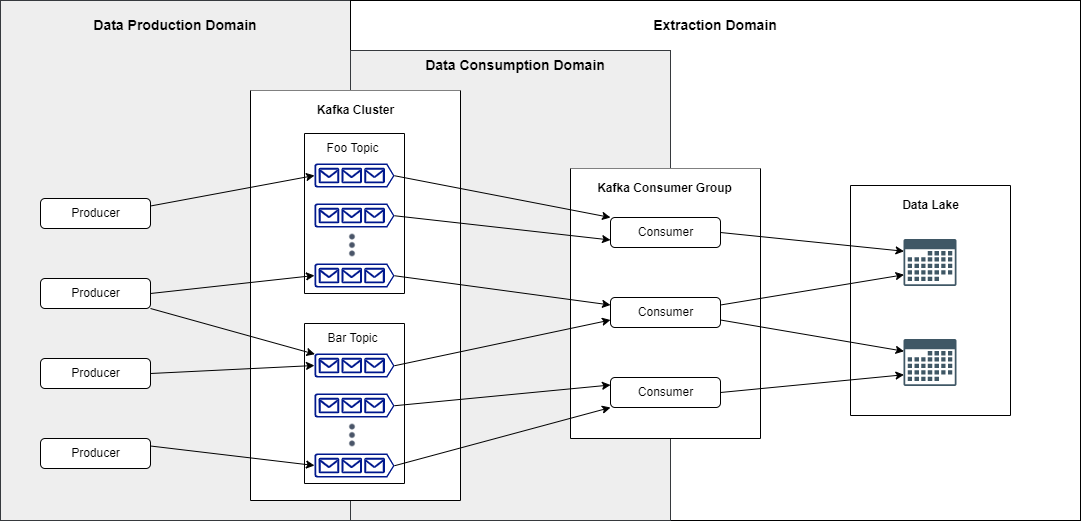
\includegraphics[width=\textwidth]{images/introduction/Context.png}
\caption{
    Data pipeline representing the flow of data since it is appended into one of
    the data sources (Topic), to when it is fetched by a consumer and inserted
    into a Data Lake.
}
\label{fig:problem_context}
\end{figure}

Throughout this work, we use Kafka as the message broker system. A Kafka cluster
is made of topics, which in turn is a unit that is subdivided into several logs,
commonly reffered to as partitions. When a producer sends a record to a specific
topic, it will be appended into one of the topic's partitions, illustrated in
the Data Production Domain in Figure \ref{fig:problem_context}. 

A consumer group is a unit composed of multiple consumers, each with the common
task of consuming data from the topics the group is subscribed to. To consume
the data within a topic, each of its partitions have to be assigned a single
consumer belonging to the same group. Assigning the partition's to different
consumers in a group, is Kafka's way of providing scalability. This design
feature leads to the fact that a group does not require more consumers than the
number of partitions, as only one consumer in a group can read data from a given
partition.

The problem was proposed by the data engineering team at HUUB (MAERSK), and it
is framed within the scope of the Extraction Domain in Figure
\ref{fig:problem_context}. It consists of being capable to dynamically manage a
group of consumers, to up- and down-scale the number of instances (i.e.
consumers), and also specify the tasks (partitions) that are assigned to each
consumer. We need to define the required amount of parallelism as to guarantee the
number of unread messages by the group does not increase with time. Hence, the
rate at which the group is consuming data from each partition, must be bigger or
equal to their respective write speed.

Considering consumers as bins, and partitions as items that have to be assigned
a bin, we model this problem as the Bin Packing Problem (BPP), with the
particularity that items vary in size with time. This occurs because the
partition's size correlates to its current write speed, which fluctuates based
on the current system's load and inevitably implies that a solution for a given
time instant may not hold true in future instants. 

On account of this BPP variation, a new solution has to be computed at each
instant, which might lead to a partition (item) being assigned to a different
consumer (bin) when compared to the consumer group's previous configuration.
Since two consumers cannot read from the same partition concurrently, the cost
associated to rebalancing a partition is related to the amount of data that is
not being read while the partition is being assigned to another consumer. 

Given that it is the first time the Bin Packing Problem is applied in this
context, existing algorithms do not take the rebalancing cost into account.
Hence, in Section \ref{sub:rscore} we propose a metric to account for a given
iteration's rebalance cost (Rscore). Additionally, using the Rscore, in Section
\ref{subsub:modified_any_fit} we propose four new BPP heuristic algorithms that
account for the rebalance costs.

The algorithms' performance is compared in section \ref{c3subsub:testing}. Since
the algorithms are attempting to solve a multi-objective problem that aims to
minimize both the number of bins required and the rebalance cost for a single
iteration, we compute the pareto front. It shows that three of the proposed
algorithms are a competitive solution to the problem at hand.

To deliver a fully automated solution to the autoscaling problem, in Chapter
\ref{chap:consumer_group_autoscaler} we introduce a system comprising three
components: a monitor, a consumer and a controller. Using the data from the
monitor process the controller uses the aforementioned theoretical approaches
(BBP heuristics) to assign tasks to consumers. Each of the components is
unitarily tested throughout Sections \ref{component:Monitor},
\ref{component:consumer} and \ref{component:controller}. An integration test is
also presented in Chapter \ref{chap:integration_tests}, aimed to reflect the
autoscaler's response time to the message broker's current load. Lastly, in
Chapter \ref{chap:conclusions}, we discuss results and suggest future work.
The following chapters introduce this thesis' technological and theoretical
background, Chapter \ref{chap:infrastructure} and Chapter \ref{chap:literature
review} respectively.


